\documentclass[10pt]{article}

\usepackage{fullpage}

\usepackage{tikz}

\usetikzlibrary{shapes.geometric, arrows}

\setlength{\parindent}{0pt}

\tikzstyle{boxEmulate} = [rectangle, rounded corners,  text width=4cm, minimum width=3cm, minimum height=1cm, text centered, draw=black, fill=white]

\tikzstyle{boxUtils} = [rectangle, rounded corners,  text width=6cm, minimum width=3cm, minimum height=1cm, draw=black, fill=white]

\tikzstyle{arrow} = [thick, ->, >=stealth]

\begin{document}

\title{\vspace{-2cm}ARM-11 CHECKPOINT}

\date{}
 
\author{Alex Richardson, Luqman Liaquat, Morkus Salasevicius, Sanchit Ajmera}

\maketitle

\section*{Introduction}
Our first course of action for this project was to decide which technologies we will use to manage our tasks and keep track of our progress. After trialling a few different options, including the Microsoft Teams Planner, we decided to use the
\textsl{‘Issues’} feature within GitLab. \textsl{Issues} allowed us to keep track of both our tasks and code progress in one place, which made the delegation and completion of tasks more streamlined. Being well-coordinated was a priority in our plan for this project as it meant we could effectively carry out our tasks and successfully build up the project. We also had regular meetings, via Discord, to discuss each member’s plans for the project, what they had completed and what they intended to complete by the end of each day.

\section*{Task Delegation}
We collectively decided to begin creating our own implementations of the foundations for this project. This included how the registers and memory were to be defined within our code. Upon completion of this initial task, we had a meeting on which features from each member’s code we will use in the project. After confirming our memory and register design, we created a list of tasks which were then split among the group. These tasks were naturally divided into three types: \textsl{Fetch, Decode} and \textsl{Execute}.
\\

The \textsl{'Fetch'} task was to generate several functions which handled the loading of the binary file and initialised
the state of our emulator. The \textsl{‘Decode’} task was to deduce the type of instruction that was loaded. The \textsl{‘Execute’} task was split further into four types based on each of the four instructions that were to be implemented. We decided to have one member working solely on the \textsl{Data Processing Instruction} and another for the \textsl{Single Data Transfer Instructions} as they required more time to complete. The \textsl{Multiply} and \textsl{Branch} instructions were relatively shorter and only needed one member to implement both functions.


\section*{Current Evaluation}
As a team, we feel that we have worked well together so far. Any conflicts on plans for a feature were solved quickly, and we have not had any issues with the work ethic of any member. Our team has been using Git to constantly commit changes with useful messages, create branches to prevent problems in the Master and updating the Git \textsl{issues}, which all translates to a well-structured process in tackling this project.
\\

The cohesive nature of our group is supported by the extensive internal code reviews we conduct for our fellow members’ tasks. To ensure that we remove logical errors within our programs and improve the definitions of some functions, we decided to work on reviewing and testing each other’s code. Although the reviews took many hours on some occasions, each member of the group was happy to help another. This meant that our overall implementation improved immensely. The reviews are an aspect of our group working that we are proud of and hope to maintain throughout this project.
\\

During the first few days, we had a problem with the group's sleeping patterns. This staggered timing meant it was harder for us to communicate effectively and work on the project together. However, after a constructive meeting, we solved that problem and had every member available to work on the project together.
\\

There are a few improvements we would like to make for future tasks. Firstly, we aim to produce our own tests \textsl{before} attempting to complete some functions, so we are confident about the expected results. We also plan to include the names of all collaborators on our future git commits, as we weren't fully consistent with this.  

\section*{Emulator Implementation}
Our aim in designing the structure of the Emulator was to ensure that it was as clear as possible for an external programmer to understand how our code worked and where everything could be found. This was achieved by maintaining a consistent naming convention, splitting files, and effectively commenting our code.


We decided to alter the initial structure of the project by incorporating additional files. This was necessary as having all our code in one place was both difficult to work on and difficult for someone else to understand. As a result, our {\tt emulate.c} file only consisted of the {\tt main} function which initialised the emulator. We extracted the remainder of the code into a new file called {\tt emulate\_utils.c}. This also removed the conflict between the main functions in our {\tt testme.c} and {\tt emulate.c} files.
 \\

We found that our code quickly became unreadable and difficult to comprehend with \textsl{‘magic numbers’} used for masks and shifts within our functions. We eliminated this issue by having sensibly named pre-processor constants at the top of our file. However, even this became too cluttered, and a better solution was needed to uphold clarity and readability within the program. This led us to create a new header file, {\tt constants.h}, which housed all the constants that were used in our Emulator. These constants were grouped by where and how they were used, which were indicated by comments. The following diagram provides a brief overview of our project structure for the emulator and includes the
general contents of each file:

\vspace{0.5cm}

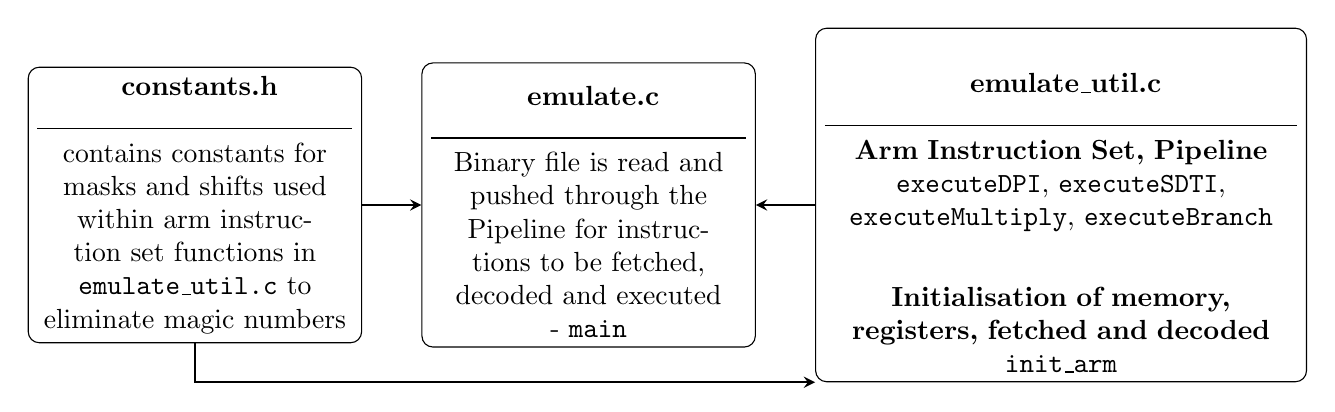
\begin{tikzpicture}[node distance=2cm]

\node (constants) [boxEmulate] {
\textbf{ constants.h} 
\rule{\textwidth}{0.4pt}
contains constants for masks and shifts used within arm instruction set functions in {\tt emulate\_util.c} to eliminate magic numbers

};

\node (emulate) [boxEmulate, right of=constants, xshift=3cm] {

\textbf{ emulate.c} 
\rule{\textwidth}{0.4pt}
Binary file is read and pushed through the Pipeline for instructions to be fetched, decoded and executed\\
 - {\tt main}

};

\node[boxUtils,xshift = 4cm, right of=emulate](emulateutil){
\center\textbf{ emulate\_util.c}
\rule{\textwidth}{0.4pt}

\textbf{Arm Instruction Set, Pipeline} \\
{\tt executeDPI},    
 {\tt executeSDTI}, 
 {\tt executeMultiply}, 
 {\tt executeBranch}\\
\vspace{0.3cm}

\vspace{0.3cm}
\textbf{Initialisation of memory, registers, fetched and decoded}\\
 {\tt init\_arm}

};

\draw [arrow] (emulateutil.west) -- (emulate.east);
\draw [arrow] (constants.east) -- (emulate.west);
\draw [arrow] (constants.south) |- (emulateutil.south west) ;

\end{tikzpicture}


\section*{Plans for the Assembler}
After discussing our plans for the assembler, we found that there are some parts of the Emulator which could be reused partly. One crucial component that will be reused is our {\tt constants.h} file which will again eliminate any magic numbers. The instruction-specific mask and shift constants will also be useful in the functions for assembling each instruction. The general structure of our instruction functions will be helpful when planning and designing our corresponding assembler functions. Finally, our error checking functions, such as the \textsl{pointer validate} function, could be reused to defend against common errors.
\\ 

An implementation task we may find challenging is creating an efficient ADT for the symbol table. We will mitigate this problem by carrying out effective research and using the lectures to their full extent. Implementing the tokenizer could be another difficult task. However, we will mitigate this problem by considering our previous projects and labs, such as the Java Spreadsheet Lab, and applying similar techniques to produce a solution. In general, our method to mitigate difficult implementation tasks consists of working together, code reviews and research. 
\end{document}
